\documentclass[tikz,border=2pt]{standalone}
\usepackage[T1]{fontenc}
\usepackage{newtxtext,newtxmath}
\usepackage{tikz}
\usetikzlibrary{positioning,arrows.meta,fit,backgrounds,calc}
\definecolor{ink}{HTML}{14202E}
\definecolor{muted}{HTML}{4A5568}
\definecolor{novo}{HTML}{A1440C}
\definecolor{gof}{HTML}{7B6CB5}
\definecolor{luz}{HTML}{1F7AA0}
\begin{document}
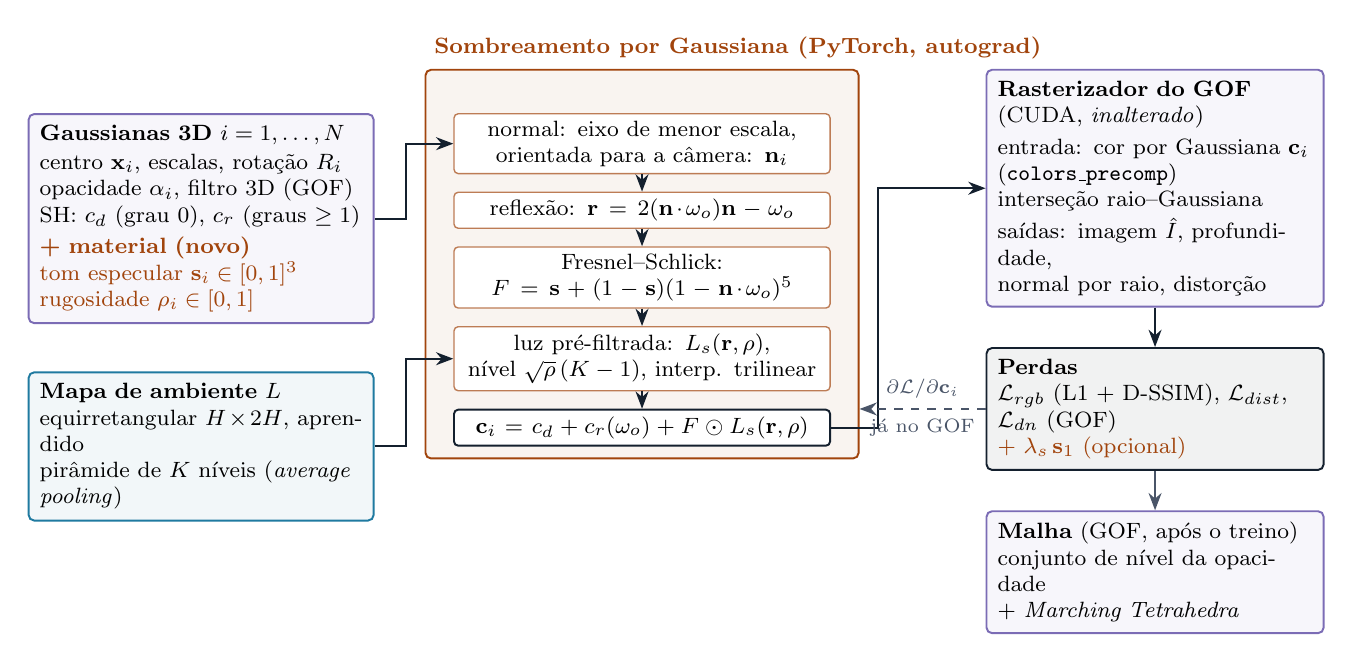
\begin{tikzpicture}[
  font=\footnotesize, >={Stealth[length=2.2mm]}, node distance=4mm and 7mm,
  caixa/.style={draw=#1, line width=0.7pt, rounded corners=2pt, align=left, inner sep=4pt, fill=#1!6, font=\footnotesize\raggedright},
  passo/.style={draw=novo!70, line width=0.5pt, rounded corners=1.5pt, align=center, inner sep=2.5pt, fill=white, text width=46mm},
  titulo/.style={font=\footnotesize\bfseries, text=ink},
  fluxo/.style={->, line width=0.7pt, draw=ink},
  grad/.style={->, line width=0.7pt, draw=muted, dashed}]

% Gaussianas e seus atributos
\node[caixa=gof, text width=41mm] (gauss) {%
  {\bfseries Gaussianas 3D} $i=1,\dots,N$\\[1pt]
  centro $\mathbf{x}_i$, escalas, rotação $R_i$\\
  opacidade $\alpha_i$, filtro 3D (GOF)\\
  SH: $c_d$ (grau 0), $c_r$ (graus $\geq 1$)\\[2pt]
  \textcolor{novo}{\bfseries + material (novo)}\\
  \textcolor{novo}{tom especular $\mathbf{s}_i\in[0,1]^3$}\\
  \textcolor{novo}{rugosidade $\rho_i\in[0,1]$}};

\node[caixa=luz, text width=41mm, below=6mm of gauss] (env) {%
  {\bfseries Mapa de ambiente} $L$\\
  equirretangular $H\times 2H$, aprendido\\ pirâmide de $K$ níveis (\emph{average pooling})};

% Sombreamento
\node[passo, right=10mm of gauss.north east, anchor=north west] (n) {normal: eixo de menor escala,\\ orientada para a câmera: $\mathbf{n}_i$};
\node[passo, below=2.2mm of n] (r) {reflexão: $\mathbf{r}=2(\mathbf{n}\!\cdot\!\omega_o)\mathbf{n}-\omega_o$};
\node[passo, below=2.2mm of r] (f) {Fresnel--Schlick:\\ $F=\mathbf{s}+(1-\mathbf{s})(1-\mathbf{n}\!\cdot\!\omega_o)^5$};
\node[passo, below=2.2mm of f] (l) {luz pré-filtrada: $L_s(\mathbf{r},\rho)$,\\ nível $\sqrt{\rho}\,(K-1)$, interp. trilinear};
\node[passo, below=2.2mm of l, draw=ink, line width=0.7pt] (c) {$\mathbf{c}_i=c_d+c_r(\omega_o)+F\odot L_s(\mathbf{r},\rho)$};
\begin{scope}[on background layer]
\node[caixa=novo, fit=(n)(c), inner sep=3.5mm, yshift=2mm] (shade) {};
\end{scope}
\node[titulo, anchor=south west, text=novo] at (shade.north west) {Sombreamento por Gaussiana (PyTorch, autograd)};

% Rasterizador
\node[caixa=gof, text width=40mm, right=16mm of shade.north east, anchor=north west] (rast) {%
  {\bfseries Rasterizador do GOF}\\ (CUDA, \emph{inalterado})\\[2pt]
  entrada: cor por Gaussiana $\mathbf{c}_i$\\ (\texttt{colors\_precomp})\\
  interseção raio--Gaussiana\\[2pt]
  saídas: imagem $\hat{I}$, profundidade,\\ normal por raio, distorção};
\node[caixa=ink, text width=40mm, below=5mm of rast] (loss) {%
  {\bfseries Perdas}\\
  $\mathcal{L}_{rgb}$ (L1 + D-SSIM), $\mathcal{L}_{dist}$, $\mathcal{L}_{dn}$ (GOF)\\
  \textcolor{novo}{$+\ \lambda_s\,\lVert\mathbf{s}\rVert_1$ (opcional)}};
\node[caixa=gof, text width=40mm, below=5mm of loss] (mesh) {%
  {\bfseries Malha} (GOF, após o treino)\\ conjunto de nível da opacidade\\ + \emph{Marching Tetrahedra}};

% Fluxos
\draw[fluxo] (gauss.east) -- ++(4mm,0) |- (n.west);
\draw[fluxo] (env.east) -- ++(4mm,0) |- (l.west);
\draw[fluxo] (n) -- (r);
\draw[fluxo] (r) -- (f);
\draw[fluxo] (f) -- (l);
\draw[fluxo] (l) -- (c);
\draw[fluxo] (c.east) -- ++(6mm,0) |- (rast.west);
\draw[fluxo] (rast) -- (loss);
\draw[fluxo, draw=muted] (loss) -- (mesh);
\draw[grad] (loss.west) -- node[above, align=center, text=muted, font=\scriptsize] {$\partial\mathcal{L}/\partial\mathbf{c}_i$} node[below, align=center, text=muted, font=\scriptsize] {já no GOF} (loss.west -| shade.east);
\end{tikzpicture}
\end{document}
